
% ==================================================
%	Durchführung
% ==================================================

\section{Durchführung}
In diesem Versuch stehen drei Koaxialkabel (20m-,50 $\Omega$; 50m-,75 $\Omega$)
zur
Verfügung. Außerdem ein Oszilloskop, ein Nim-Pulser und diverse
Abschlusswiderstände.

\begin{figure}[htpb]
  \centering
  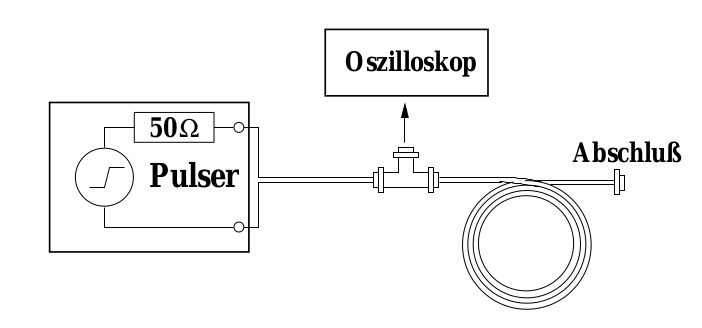
\includegraphics[scale=1.0]{bilder/aufbau.png}
  \caption{Aufbau.}
\label{fig:aufbau}
\end{figure}

\begin{enumerate}
\item 	Es wird ein LRC-Messgerät an das 20m-Koaxialkabel angeschlossen, und die
		Leitungskonstanten $R$, $L$ und $C$ in Abhängigkeit von der angelegten
		Frequenz gemessen. Dabei ist das andere Ende des Kabels kurzgeschlossen.

\item 	Der Aufbau geschieht nun nach Abbildung \ref{fig:Aufbau}.
		Die Dämpfungskonstante $\alpha$ wird für die drei Koaxialkabel bestimmt.
		Dazu wird ein Eingangsimpuls (Nim-Pulser) mit hohem Oberwellenanteil
		benutzt, und die
		Fourierkoeffizienten der Oberwellen gemessen.

\item 	An einem Koaxialkabel mit zuerst offenem, dann kurzgeschlossenem Ende
		werden die Eingangsimpedanzen gemessen.

\item	Es werden
		nacheinander drei Abschlusswiderstände unbekannter Eingenschaft
		angeschlossen und das Bild am Oszilloskop aufgenommen.

\item	Das $50 \,\Omega$ und $75 \, \Omega$ Kabel werden in Reihe geschaltet und
		das	Oszilloskopbild aufgenommen.


\end{enumerate}

